\documentclass[tikz, border=3mm]{standalone}
\usepackage{tikz}
\usetikzlibrary{arrows.meta} % For arrow tips

\begin{document}
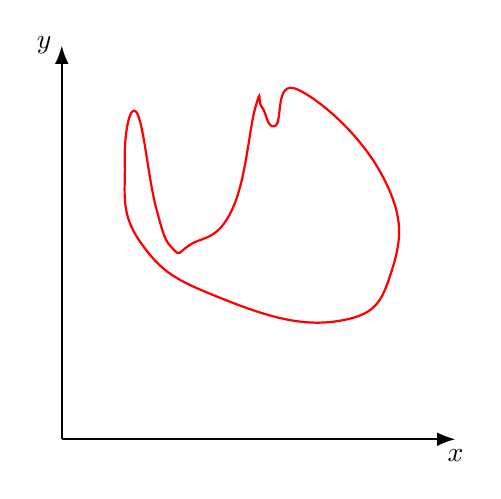
\begin{tikzpicture}[
    >=Latex, % Set default arrow tip style
    axis/.style={->, thick} % Style for axes
]

    % Axes (adjust limits to fit the new coordinates)
    \draw[axis] (0, 0) -- (5, 0) node[below] {$x$};
    \draw[axis] (0, 0) -- (0, 5) node[left] {$y$};

    % Draw the Red Curve using the specified coordinates
    \draw[red, thick] plot [smooth cycle, tension=0.8] coordinates {
        (0.95, 4.15)
        (1.2, 2.93)
        (1.41, 2.42)
        (1.63, 2.47)
        (2.16, 2.91)
        (2.46, 4.22)
        (2.54, 4.22) % Note: Duplicate x-value, slight y change
        (2.71, 3.98)
        (3.0, 4.44)  % Highest y-value
        (4.08, 3.33)
        (4.19, 2.14) % Lowest y-value, Rightmost x-value
        % Add more points here if needed to close the loop smoothly back to (0.95, 4.15)
        % For example, adding points to bring it down and left:
        (3.5, 1.5)
        (2.0, 1.8)
        (1.0, 2.5)
        (0.8, 3.5)
     }; % The 'cycle' option closes the loop

\end{tikzpicture}
\end{document}